% Nguồn SGK Toán 9 Tập hai — Luyện tập chung sau Bài 32, trang 106--107:
% https://cdn3.olm.vn/upload/thuvienso/4491669493-page-106-1771844569948.png
% https://cdn3.olm.vn/upload/thuvienso/4491669493-page-107-1771844570287.png

\section*{Luyện tập chung}

\begin{exercises}
    \textbf{Ví dụ 1}

    Một hình trụ có bán kính đáy bằng $1$ cm và chiều cao bằng $2$ cm. Người ta khoan một phần có dạng hình nón như Hình 10.28 thì thể tích phần còn lại của hình trụ bằng bao nhiêu?

    \begin{center}
        \begin{tikzpicture}
            \coordinate (TopCenter) at (0,2.4);
            \coordinate (BottomCenter) at (0,0);
            \coordinate (TopLeft) at (-1.15,2.4);
            \coordinate (TopRight) at (1.15,2.4);
            \coordinate (BottomLeft) at (-1.15,0);
            \coordinate (BottomRight) at (1.15,0);

            \draw (TopCenter) ellipse [x radius=1.15cm, y radius=0.32cm];
            \draw (TopLeft)--(BottomLeft);
            \draw (TopRight)--(BottomRight);
            \draw (BottomLeft) arc[start angle=180,end angle=360,x radius=1.15cm,y radius=0.32cm];
            \draw[dashed] (BottomRight) arc[start angle=0,end angle=180,x radius=1.15cm,y radius=0.32cm];
            \draw[dashed] (TopLeft)--(BottomCenter)--(TopRight);
            \draw (BottomCenter)--(BottomRight) node[midway,below] {$1$ cm};
            \node[right=4pt of $(TopRight)!0.5!(BottomRight)$] {$2$ cm};
        \end{tikzpicture}

        \textit{Hình 10.28}
    \end{center}

    \textbf{Giải}

    Thể tích của hình trụ là $V_1=\pi R^2h=\pi\cdot 1^2\cdot 2=2\pi$ (cm$^3$).

    Thể tích phần bị khoan có dạng hình nón là:
    \[
        V_2=\dfrac{1}{3}\pi R^2h=\dfrac{1}{3}\pi\cdot 1^2\cdot 2=\dfrac{2\pi}{3}\text{ (cm}^3\text{)}.
    \]

    Thể tích phần còn lại là $V=V_1-V_2=2\pi-\dfrac{2\pi}{3}=\dfrac{4\pi}{3}$ (cm$^3$).

    \textbf{Ví dụ 2}

    Một hộp đựng bóng tennis có dạng hình trụ chứa vừa khít ba quả bóng tennis xếp theo chiều dọc (H.10.29). Các quả bóng tennis có dạng hình cầu, đường kính $6{,}4$ cm.
    \begin{enumerate}[label=\alph*)]
        \item Tính thể tích hộp đựng bóng (bỏ qua bề dày của vỏ hộp, làm tròn kết quả đến hàng đơn vị của cm$^3$).
        \item Tính thể tích bên trong hộp đựng bóng không bị chiếm bởi ba quả bóng tennis.
    \end{enumerate}

    \begin{center}
        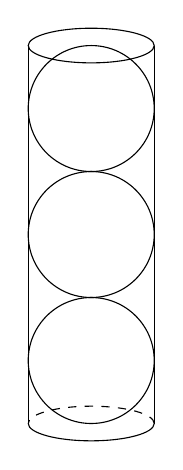
\begin{tikzpicture}
            \coordinate (TopCenter) at (0,4.8);
            \coordinate (BottomCenter) at (0,0);
            \coordinate (TopLeft) at (-0.8,4.8);
            \coordinate (TopRight) at (0.8,4.8);
            \coordinate (BottomLeft) at (-0.8,0);
            \coordinate (BottomRight) at (0.8,0);
            \coordinate (BallOne) at (0,0.8);
            \coordinate (BallTwo) at (0,2.4);
            \coordinate (BallThree) at (0,4.0);

            \draw (TopCenter) ellipse [x radius=0.8cm, y radius=0.22cm];
            \draw (TopLeft)--(BottomLeft);
            \draw (TopRight)--(BottomRight);
            \draw (BottomLeft) arc[start angle=180,end angle=360,x radius=0.8cm,y radius=0.22cm];
            \draw[dashed] (BottomRight) arc[start angle=0,end angle=180,x radius=0.8cm,y radius=0.22cm];
            \draw (BallOne) circle[radius=0.8cm];
            \draw (BallTwo) circle[radius=0.8cm];
            \draw (BallThree) circle[radius=0.8cm];
        \end{tikzpicture}

        \textit{Hình 10.29}
    \end{center}

    \textbf{Giải}

    \begin{enumerate}[label=\alph*)]
        \item Chiều cao hộp đựng bóng hình trụ là $h=6{,}4\cdot 3=19{,}2$ (cm).

        Bán kính đáy hộp đựng bóng hình trụ là $R=6{,}4:2=3{,}2$ (cm).

        Thể tích hộp đựng bóng hình trụ nói trên là:
        \[
            V=\pi R^2h=\pi\cdot 3{,}2^2\cdot 19{,}2\approx 618\text{ (cm}^3\text{)}.
        \]

        \item Bán kính quả bóng tennis là $R'=6{,}4:2=3{,}2$ (cm).

        Thể tích của ba quả bóng tennis nói trên là:
        \[
            V'=3\cdot\left(\dfrac{4}{3}\cdot\pi R'^3\right)=3\cdot\left(\dfrac{4}{3}\cdot\pi\cdot 3{,}2^3\right)\approx 412\text{ (cm}^3\text{)}.
        \]

        Thể tích bên trong hộp đựng bóng không bị chiếm bởi ba quả bóng tennis là:
        \[
            V''=V-V'\approx 618-412=206\text{ (cm}^3\text{)}.
        \]
    \end{enumerate}

    \subsection{Bài tập}

    \begin{questions}[resume=SGK]
        \item Cho một hình trụ có đường kính của đáy bằng với chiều cao và có thể tích bằng $2\pi$ cm$^3$.
        \begin{questions}
            \item Tính chiều cao của hình trụ.

            \answerline
            \answerline

            \item Diện tích toàn phần của hình trụ bằng tổng diện tích xung quanh và diện tích hai đáy hình trụ. Tính diện tích toàn phần của hình trụ trên.

            \answerline
            \answerline
            \answerline
        \end{questions}

        \item Một vòng bi bằng thép (phần thép giữa hai hình trụ) có hình dạng và kích thước như Hình 10.30. Tính thể tích của vòng bi đó.

        \begin{center}
            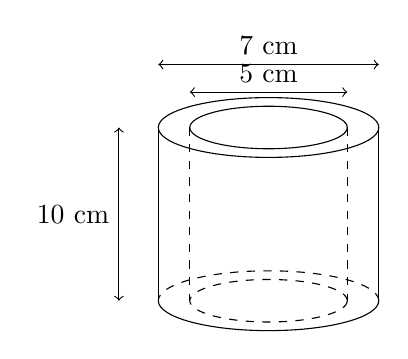
\begin{tikzpicture}
                \coordinate (OuterTopCenter) at (0,2.2);
                \coordinate (OuterBottomCenter) at (0,0);
                \coordinate (OuterTopLeft) at (-1.4,2.2);
                \coordinate (OuterTopRight) at (1.4,2.2);
                \coordinate (OuterBottomLeft) at (-1.4,0);
                \coordinate (OuterBottomRight) at (1.4,0);
                \coordinate (InnerTopCenter) at (0,2.2);
                \coordinate (InnerBottomCenter) at (0,0);
                \coordinate (InnerTopLeft) at (-1.0,2.2);
                \coordinate (InnerTopRight) at (1.0,2.2);

                \draw (OuterTopCenter) ellipse[x radius=1.4cm,y radius=0.38cm];
                \draw (InnerTopCenter) ellipse[x radius=1.0cm,y radius=0.27cm];
                \draw (OuterTopLeft)--(OuterBottomLeft);
                \draw (OuterTopRight)--(OuterBottomRight);
                \draw (OuterBottomLeft) arc[start angle=180,end angle=360,x radius=1.4cm,y radius=0.38cm];
                \draw[dashed] (OuterBottomRight) arc[start angle=0,end angle=180,x radius=1.4cm,y radius=0.38cm];
                \draw[dashed] (InnerTopLeft)--(-1.0,0);
                \draw[dashed] (InnerTopRight)--(1.0,0);
                \draw[dashed] (InnerBottomCenter) ellipse[x radius=1.0cm,y radius=0.27cm];

                \draw[<->] (-1.4,3.0)--(1.4,3.0) node[midway,above] {$7$ cm};
                \draw[<->] (-1.0,2.65)--(1.0,2.65) node[midway,above] {$5$ cm};
                \draw[<->] (-1.9,0)--(-1.9,2.2) node[midway,left] {$10$ cm};
            \end{tikzpicture}

            \textit{Hình 10.30}
        \end{center}

        \answerline
        \answerline
        \answerline

        \item Chiếc mũ của chú hề với các kích thước như Hình 10.31. Hãy tính tổng diện tích vải cần để làm chiếc mũ (coi mép khâu không đáng kể và làm tròn kết quả đến hàng phần mười của cm$^2$).

        \begin{center}
            \begin{tikzpicture}
                \coordinate (Apex) at (0,3.9);
                \coordinate (ConeBaseCenter) at (0,0.75);
                \coordinate (ConeBaseLeft) at (-0.9,0.75);
                \coordinate (ConeBaseRight) at (0.9,0.75);
                \coordinate (BrimCenter) at (0,0.55);
                \coordinate (BrimLeft) at (-2.1,0.55);
                \coordinate (BrimRight) at (2.1,0.55);

                \draw (Apex)--(ConeBaseLeft);
                \draw (Apex)--(ConeBaseRight);
                \draw (ConeBaseCenter) ellipse[x radius=0.9cm,y radius=0.22cm];
                \draw (BrimCenter) ellipse[x radius=2.1cm,y radius=0.5cm];
                \draw[dashed] (ConeBaseLeft) arc[start angle=180,end angle=360,x radius=0.9cm,y radius=0.22cm];

                \draw[<->] ($(Apex)!0.05!(ConeBaseRight)+(0.25,0)$)--($(Apex)!0.95!(ConeBaseRight)+(0.25,0)$) node[midway,right] {$30$ cm};
                \draw[<->] (BrimLeft)--(ConeBaseLeft) node[midway,below] {$10$ cm};
                \draw[<->] (-2.1,-0.35)--(2.1,-0.35) node[midway,below] {$35$ cm};
            \end{tikzpicture}

            \textit{Hình 10.31}
        \end{center}

        \answerline
        \answerline
        \answerline
        \answerline

        \item Người ta nhấn chìm hoàn toàn $5$ viên bi có dạng hình cầu vào một chiếc cốc hình trụ đựng đầy nước, mỗi viên bi có đường kính $2$ cm. Tính lượng nước tràn ra khỏi cốc.

        \answerline
        \answerline
        \answerline

        \item Một bồn chứa xăng gồm hai nửa hình cầu có đường kính bằng $1{,}8$ m và một hình trụ có chiều cao bằng $3{,}6$ m (H.10.32). Tính thể tích của bồn chứa xăng (làm tròn kết quả đến hàng phần trăm của m$^3$).

        \begin{center}
            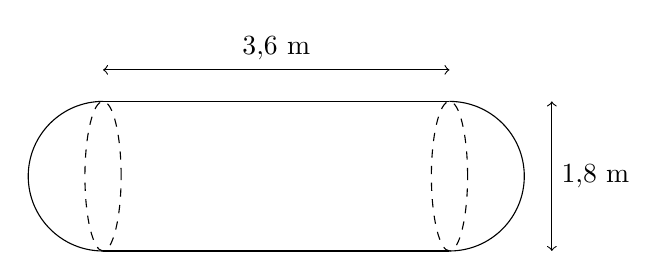
\begin{tikzpicture}
                \coordinate (LeftCenter) at (-2.2,0);
                \coordinate (RightCenter) at (2.2,0);
                \coordinate (LeftTop) at (-2.2,0.95);
                \coordinate (LeftBottom) at (-2.2,-0.95);
                \coordinate (RightTop) at (2.2,0.95);
                \coordinate (RightBottom) at (2.2,-0.95);

                \draw (LeftTop)--(RightTop);
                \draw (LeftBottom)--(RightBottom);
                \draw (LeftTop) arc[start angle=90,end angle=270,x radius=0.95cm,y radius=0.95cm];
                \draw (RightBottom) arc[start angle=-90,end angle=90,x radius=0.95cm,y radius=0.95cm];
                \draw[dashed] (LeftCenter) ellipse[x radius=0.23cm,y radius=0.95cm];
                \draw[dashed] (RightCenter) ellipse[x radius=0.23cm,y radius=0.95cm];
                \draw[<->] (-2.2,1.35)--(2.2,1.35) node[midway,above] {$3{,}6$ m};
                \draw[<->] (3.5,-0.95)--(3.5,0.95) node[midway,right] {$1{,}8$ m};
            \end{tikzpicture}

            \textit{Hình 10.32}
        \end{center}

        \answerline
        \answerline
        \answerline
        \answerline

        \item Từ một tấm tôn hình chữ nhật có kích thước $50$ cm $\times$ $240$ cm, người ta làm mặt xung quanh của các thùng đựng nước hình trụ có chiều cao bằng $50$ cm, theo hai cách sau (H.10.33):

        \begin{itemize}
            \item \textit{Cách 1:} Gò tấm tôn ban đầu thành mặt xung quanh của thùng nước hình trụ.
            \item \textit{Cách 2:} Cắt tấm tôn ban đầu thành hai tấm hình chữ nhật bằng nhau, rồi gò mỗi tấm đó thành mặt xung quanh của một thùng.
        \end{itemize}

        Kí hiệu $V_1$ là thể tích của thùng gò được theo \textit{Cách 1} và $V_2$ là tổng thể tích của hai thùng gò được theo \textit{Cách 2}. Tính tỉ số $\dfrac{V_1}{V_2}$ (giả sử các mối hàn là không đáng kể).

        \begin{center}
            \begin{tikzpicture}
                \coordinate (OneRectBL) at (-3.0,1.6);
                \coordinate (OneRectTR) at (0.2,2.5);
                \coordinate (OneCylinderCenter) at (3.2,2.05);
                \coordinate (TwoRectBL) at (-3.0,-0.4);
                \coordinate (TwoRectTR) at (0.2,0.5);
                \coordinate (TwoCylinderTop) at (2.7,0.35);
                \coordinate (TwoCylinderBottom) at (3.7,-0.25);

                \node[left=8pt of OneRectBL] {\textit{Cách 1:}};
                \draw (OneRectBL) rectangle (OneRectTR);
                \draw[-{Stealth[length=3mm,width=2.2mm]}] (0.5,2.05)--(1.6,2.05);
                \draw (2.25,1.5) ellipse[x radius=0.75cm,y radius=0.2cm];
                \draw (1.5,1.5)--(1.5,2.55);
                \draw (3.0,1.5)--(3.0,2.55);
                \draw (2.25,2.55) ellipse[x radius=0.75cm,y radius=0.2cm];
                \draw (1.5,1.5) arc[start angle=180,end angle=360,x radius=0.75cm,y radius=0.2cm];
                \draw[dashed] (3.0,1.5) arc[start angle=0,end angle=180,x radius=0.75cm,y radius=0.2cm];

                \node[left=8pt of TwoRectBL] {\textit{Cách 2:}};
                \draw (TwoRectBL) rectangle (TwoRectTR);
                \draw[dashed] (-1.4,-0.4)--(-1.4,0.5);
                \draw[-{Stealth[length=3mm,width=2.2mm]}] (0.5,0.05)--(1.6,0.05);

                \draw (2.2,-0.45) ellipse[x radius=0.55cm,y radius=0.16cm];
                \draw (1.65,-0.45)--(1.65,0.35);
                \draw (2.75,-0.45)--(2.75,0.35);
                \draw (2.2,0.35) ellipse[x radius=0.55cm,y radius=0.16cm];
                \draw (1.65,-0.45) arc[start angle=180,end angle=360,x radius=0.55cm,y radius=0.16cm];
                \draw[dashed] (2.75,-0.45) arc[start angle=0,end angle=180,x radius=0.55cm,y radius=0.16cm];

                \draw (3.55,-0.45) ellipse[x radius=0.55cm,y radius=0.16cm];
                \draw (3.0,-0.45)--(3.0,0.35);
                \draw (4.1,-0.45)--(4.1,0.35);
                \draw (3.55,0.35) ellipse[x radius=0.55cm,y radius=0.16cm];
                \draw (3.0,-0.45) arc[start angle=180,end angle=360,x radius=0.55cm,y radius=0.16cm];
                \draw[dashed] (4.1,-0.45) arc[start angle=0,end angle=180,x radius=0.55cm,y radius=0.16cm];
            \end{tikzpicture}

            \textit{Hình 10.33}
        \end{center}

        \answerline
        \answerline
        \answerline
        \answerline
    \end{questions}
\end{exercises}
